\documentclass{beamer}

\usepackage{framed}
\usepackage{graphicx}

\begin{document}
\section{Visualizing pairwise relationships in a dataset}
%===========================================================%
\begin{frame}[fragile]
	\Large
\begin{itemize}
\item To plot multiple pairwise bivariate distributions in a dataset, you can use the \texttt{pairplot()} function.
\item  This creates a matrix of axes and shows the relationship for each pair of columns in a DataFrame. 
\item By default, it also draws the univariate distribution of each variable on the diagonal Axes:
\end{itemize}
\begin{verbatim}
iris = sns.load_dataset("iris")
sns.pairplot(iris);
\end{verbatim}
\end{frame}
%===========================================================%
\begin{frame}
\begin{figure}
\centering
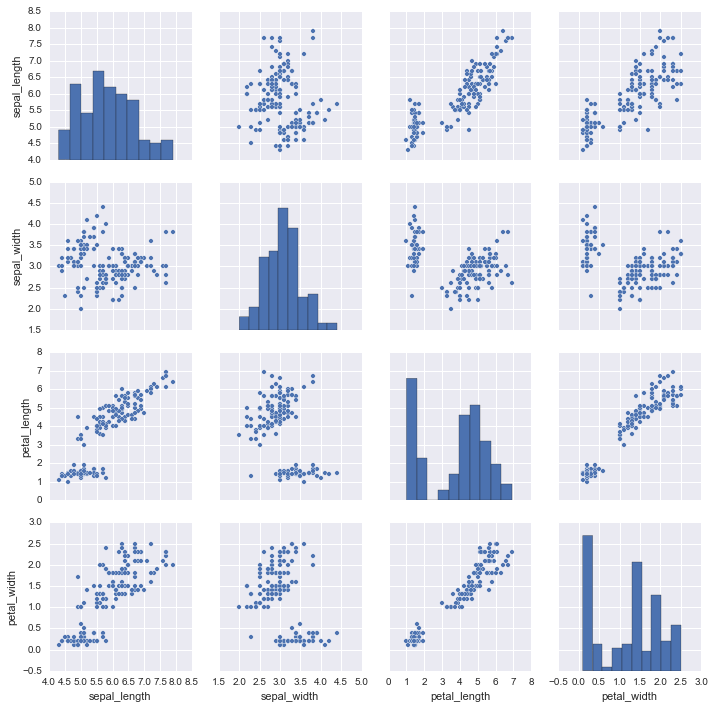
\includegraphics[width=0.8\linewidth]{images/distributions_42_0}
\caption{}
\label{fig:distributions_42_0}
\end{figure}

\end{frame}
%===========================================================%
\begin{frame}[fragile]
	\frametitle{Seaborn Workshop}
	\large
Much like the relationship between \texttt{jointplot()} and \texttt{JointGrid}, the \texttt{pairplot()} function is built on top of a \texttt{PairGrid} object, which can be used directly for more flexibility:
\begin{framed}
\begin{verbatim}
g = sns.PairGrid(iris)
g.map_diag(sns.kdeplot)
g.map_offdiag(sns.kdeplot, cmap="Blues_d", 
          n_levels=6);
\end{verbatim}
\end{framed}
\end{frame}
%========================================================= %
%/Users/mwaskom/anaconda/lib/python2.7/site-packages/matplotlib/axes/_axes.py:475: UserWarning: No labelled objects found. Use label='...' kwarg on individual plots.
%  warnings.warn("No labelled objects found. "
%../_images/distributions_44_1.png
\begin{frame}[fragile]
\begin{figure}
\centering
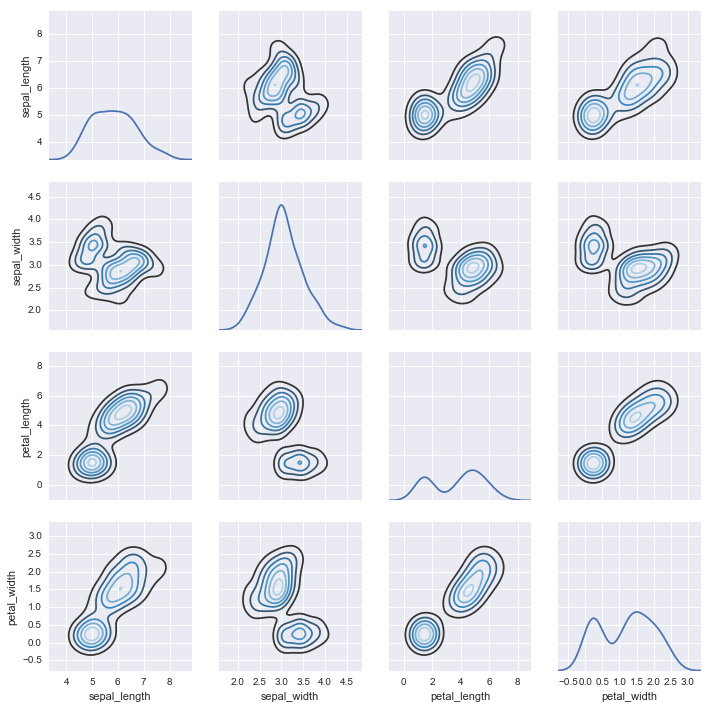
\includegraphics[width=0.7\linewidth]{images/distributions_44_1}
\end{figure}
\end{frame}

\end{document}